\documentclass{article}
\usepackage[utf8]{inputenc}
\usepackage{geometry}
 \geometry{
 a4paper,
 total={170mm,257mm},
 left=20mm,
 top=20mm,
 }
\usepackage{tikz}\usetikzlibrary{automata, positioning, arrows}

\title{ COMP 330 Winter 2021 \\ Assignment 2}
\author{Belle Pan 260839939}
\date{4th February 2021}

\usepackage{natbib}
\usepackage{graphicx}

\begin{document}

\maketitle

\noindent \textbf{Solution 1. 
\\Give regular expressions for the following languages over \(\{a,b\}\) :
\begin{enumerate}
    \item \(\{w|w\) contains an even number of occurrences of \(a\}\)
    \item \(\{w|w\) contains an odd number of occurrences of \(b\}\)
    \item \(\{w|\) does not contain the substring \(ab\}\)
    \item \(\{w|w\) does not contain the substring \(aba\}\)
\end{enumerate}}
\\
\\\noindent Below are the corresponding regular expressions:
\begin{enumerate}
    \item \((b^*ab^*ab^*)^* + b^*\)
    \item \((a^*ba^*)(ba^*ba^*)^*\)
    \item \(b^*a^*\)
    \item \(b^*+b^*aa^*(bbb^*aa^*)^*b^*\)
\end{enumerate}
\\
\\\noindent \textbf{Solution 2. 
\\Suppose you have a DFA \(M = (S, \Sigma, s_0, \delta, F)\). Consider two sitinct states \(s_1, s_2\), i.e. \(s_1 \neq s_2\). Suppose further that for all \(a\in \Sigma\) \(\delta (s_1,a) = \delta (s_2,a)\). Show that for any nonempty word \(w\) over \(\Sigma\) we have \(\delta^* (s_1,a) = \delta^* (s_2,a)\).}
\\
\\Using induction on the length of the word \(w\):
\begin{itemize}
    \item Base case: \(|w| = 1\) (length of the word \(w\) is \(1\))
    \begin{itemize}
        \item We must show that for all \(a \in \Sigma, \delta ^*(s_1,a) = \delta^* (s_2,a)\).
        \item This is already given in the question, \(\forall a\in \Sigma\) \(\delta (s_1,a) = \delta (s_2,a)\).
        \item Therefore, there is no other verification processes needed.
    \end{itemize}
    \item Inductive Hypothesis: \(\forall w\in \Sigma ^*,\) \(|w|<n\) \(\Longrightarrow\) \(\delta^* (s_1,w) = \delta^* (s_2,w)\).
    \begin{itemize}
        \item Consider a word \(wa\) where \(a\) is any letter \(\in \Sigma\) and \(|w| = n-1\).
        \item This yields : \(\delta^* (s_1,wa)\)
        \item By the definition of \(\delta ^*\), \(\delta^* (s_1,wa)= \delta(\delta^* (s_1,w),a) \).
        \item Then, by the inductive hypothesis, \(\delta^* (s_1,wa)= \delta(\delta^* (s_1,w),a) = \delta(\delta^*(s_2,w),a)\)
        \item And finally, by the definition of \(\delta ^*\), \(\delta^* (s_1,wa)= \delta(\delta^* (s_1,w),a) = \delta(\delta^*(s_2,w),a) = \delta^*(s_2,wa)\)
    \end{itemize}
\end{itemize}
The inductive hypothesis holds and thus shows that for any nonempty word \(w\) over \(\Sigma\) we have \(\delta^* (s_1,a) = \delta^* (s_2,a)\).
\\
\\\noindent \textbf{Solution 3. Show that the following languages are not regular by using the pumping lemma:
\begin{enumerate}
    \item \(\{a^nb^ma^{n+m}|n,m\geq 0\}\)
    \item \(\{x|x=x^R,x\in \Sigma ^*\}\) where \(x^R\) means \(x\) reversed (palindromes).
\end{enumerate}
}
\\\\
\noindent Below are the corresponding proofs using the demon - angel strategy of showing the pumping lemma:
\begin{enumerate}
    \item \begin{enumerate}
        \item The demon picks a number \(p\).
        \item The angel picks the word \(a^pba^{(p+1)}\).
        \item The demon is forced to pick a \(y\) value that is made of exclusively \(a\)'s due to the constraints \(|xy|\leq p\) and \(|y| > 0\). Suppose that \(y=a^k\).
        \item The angel picks \(i=3\) such that the new word is \(a^{p+2k}ba^{p+1}\). This word is not in the language as \(1 \neq 2k\).
        \item Thus, by the pumping lemma, this language is indeed not regular.
    \end{enumerate}
    \item \begin{enumerate}
        \item The demon picks a number \(p\).
        \item The angel picks the word \(a^pbba^p\).
        \item The demon is forced to pick \(x\), \(y\), \(z\) values such that for any \(i \geq 0\), \(xy'z\) remains a palindrome; thus, \(x = a^j\) for some \(j\in\{0,...,p-1\}\), \(y = a^k\) for some \(k\in \{1,...,p\}\), and \(z=a^lbba^p\) for some \(l \in \{0,...,p-1\}\).
        \item The angel picks \(i=2\) such that the new word is \(a^{p+k}bba^p\). As \(k>0\), this word is not a palindrome and is thus not in the language.
        \item Therefore, by the pumping lemma, this language is indeed not regular.
    \end{enumerate}
\end{enumerate}


\noindent \textbf{Solution 4. Show that the following languages are not regular by using the pumping lemma:
\begin{enumerate}
    \item \(\{a\in \{a,b,c\}^*||x|\) is a square\(\}\), where \(|x|\) means the length of \(x\).
    \item \(\{a^{2n}b^{n}\}\)
\end{enumerate}
\\}
\\
\\\noindent Below are the corresponding proofs using the demon - angel strategy of showing the pumping lemma:
\begin{enumerate}
    \item \begin{enumerate}
        \item The demon picks a number \(p\).
        \item The angel picks the word \(a^{p^2}\). \(|a^{p^2}|=p^2\).
        \item The demon is forced to pick a \(y\) value that is made of exclusively \(a\)'s due to the constraints \(|xy|\leq p\) and \(|y| > 0\). Let \(|y| = k\) and \(0<k\leq p\).
        \item The angel picks \(i=2\) such that the new word is \(a^{p^2+k}\) and \(|a^{p^2+k}| = p^2+k\). As \(k\leq p < p+1\), we know that \(p^2+k < p^2+2p+1 = (p+1)^2\); \(p^2+k\) cannot be a square number as it is strictly less than the square after \(4p^2\) and thus is not in the language.
        \item Therefore, by the pumping lemma, this language is indeed not regular.
    \end{enumerate}
    \item \begin{enumerate}
        \item The demon picks a number \(p\).
        \item The angel picks the word \(a^{2p}b^{p}\).
        \item The demon is forced to pick a \(y\) value that is made of exclusively \(a\)'s due to the constraints \(|xy|\leq p\) and \(|y| > 0\). Let \(|y|=k\) and \(k>0\).
        \item The angel picks \(i=0\) such that the new word is \(a^{2p-k}b^p\). As \(2p-k\neq 2p\), this word is not in the language.
        \item Thus, by the pumping lemma, this language is indeed not regular.
    \end{enumerate}
\end{enumerate}
\newpage


\noindent \textbf{Solution 5. We are using the alphabet \(\{0,1\}\). We have a DFA with 5 states, \(S = \{s_0, s_1, s_2, s_3, s_4\}\). The start state is \(s_0\) and the only accepting state is also \(s_0\). The transitions are given by the formula \(\delta(s_i,a) = s_j\) where \(j=i^2+a\) mod 5. Draw the table showing which pairs of states are in-equivalent and then construct the minimal automaton. Remember to remove useless states right from the start, before you draw the table.}
\\\\
\noindent Let us draw the automaton described:


\begin{figure}[h]
   \centering
    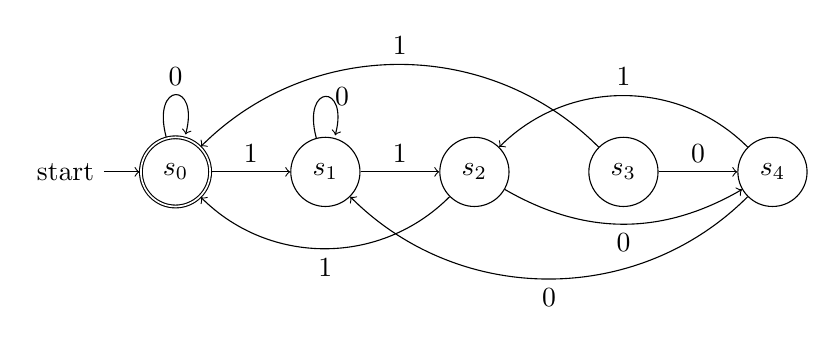
\begin{tikzpicture}
        \node[state,initial, accepting](s_0) {$s_0$};
        \node[state] (s_1) [right=of s_0] {$s_1$};
        \node[state] (s_2) [right=of s_1] {$s_2$};
        \node[state] (s_3) [right=of s_2] {$s_3$};
        \node[state] (s_4) [right=of s_3] {$s_4$};
        \path[->] 
                (s_0) edge node [above] {1} (s_1)
                    edge [loop above] node {0} ()
                (s_1) edge node [above] {1} (s_2)
                    edge [loop above] node [right] {0} ()
                (s_2) edge [bend left = 45] node [below] {1} (s_0)
                    edge [bend right] node [below] {0} (s_4)
                (s_3) edge [bend right = 45] node [above] {1} (s_0)
                    edge node [above] {0} (s_4)
                (s_4) edge [bend right=45] node [above] {1} (s_2)
                    edge [bend left=45] node [below] {0} (s_1);
    \end{tikzpicture}
\end{figure}
\noindent We notice that \(s_3\) is an unreachable state; this means that we may remove it immediately, before the table is drawn.\\

\begin{table}[h!]
    \centering
    \begin{tabular}{ |p{3cm}|p{3cm}|p{3cm}|p{3cm}|p{3cm}|}
    \hline
    
        States & \textbf{\(s_0\)} & \textbf{\(s_1\)} & \textbf{\(s_2\)}& \textbf{\(s_4\)}\\
        \hline
        \hline
        \(s_0\)  & Self   & 0   &  0  & 0\\
        \hline
        \(s_1\)&     & Self   & 0 & \textbf{1}\\
        \hline
        \(s_2\)&   & & Self   & 0\\
        \hline 
        \(s_4\)  &   &    &  & Self\\
        \hline
\end{tabular}
    \caption{The table achieved by running the algorithm.}
    \label{tab:my_label}
\end{table}
\noindent There is only one pair of states that are equivalent by the algorithm : \(s_1\) and \(s_4\). We may now create the following minimized DFA:

\begin{figure}[h]
   \centering
    \begin{tikzpicture}
        \node[state,initial, accepting](s_0) {$s_0$};
        \node[state] (s_{14}) [right=of s_0] {$s_{14}$};
        \node[state] (s_2) [right=of s_1] {$s_2$};
        \path[->] 
                (s_0) edge node [above] {1} (s_1)
                    edge [loop above] node {0} ()
                (s_{14}) edge node [below] {1} (s_2)
                    edge [loop above] node [above] {0} ()
                (s_2) edge [bend left = 45] node [below] {1} (s_0)
                    edge [bend right = 45] node [above] {0} (s_{14});
    \end{tikzpicture}
\end{figure}

\end{document}
